% Part 1: Technical Landscape
\section{Technical Landscape}

\begin{frame}
\frametitle{Transformer Architecture}
\begin{itemize}
    \item \textbf{"Attention is All You Need"} (Vaswani et al., 2017)
    \item Self-attention mechanism: captures long-range dependencies
    \item Key components:
    \begin{itemize}
        \item Multi-head attention
        \item Positional encoding
        \item Feed-forward networks
        \item Layer normalization
    \end{itemize}
    \item Advantages:
    \begin{itemize}
        \item Parallel processing (vs. sequential RNNs)
        \item Flexible context modeling
        \item Scalable architecture
    \end{itemize}
\end{itemize}
\end{frame}

\begin{frame}
\frametitle{Probabilistic Modeling}
\begin{itemize}
    \item Language modeling as probability distribution: $P(w_1, w_2, ..., w_n)$
    \item Autoregressive formulation: $P(w_t | w_1, ..., w_{t-1})$
    \item Training objectives:
    \begin{itemize}
        \item Autoregressive language modeling
        \item Masked language modeling
        \item Diffusion models
    \end{itemize}
    \item Maximum likelihood estimation via cross-entropy loss
    \item Foundation for generation and understanding
\end{itemize}
\end{frame}

\begin{frame}
\frametitle{Scaling Laws}
\begin{itemize}
    \item \textbf{Key insight}: Model performance scales predictably with:
    \begin{itemize}
        \item Model size (parameters)
        \item Dataset size (tokens)
        \item Compute budget (FLOPs)
    \end{itemize}
    \item Power law relationships (Kaplan et al., 2020)
    \item Chinchilla scaling laws (Hoffmann et al., 2022):
    \begin{itemize}
        \item Optimal ratio of model size to training data
        \item Compute-optimal training
    \end{itemize}
    \item Implications: Bigger models, more data = better performance
\end{itemize}
\end{frame}

\begin{frame}
\frametitle{Emergent Abilities}
\begin{itemize}
    \item Capabilities that appear at scale, absent in smaller models
    \item Examples:
    \begin{itemize}
        \item Few-shot learning (GPT-3)
        \item Chain-of-thought reasoning
        \item Instruction following
        \item Multi-step problem solving
        \item Arithmetic and symbolic reasoning
    \end{itemize}
    \item Not explicitly trained, emerge from scale
    \item Phase transitions in capability vs. scale
    \item Critical for advanced applications
\end{itemize}
\end{frame}

\begin{frame}
\frametitle{LLM and Agent Development Roadmap}
\begin{center}
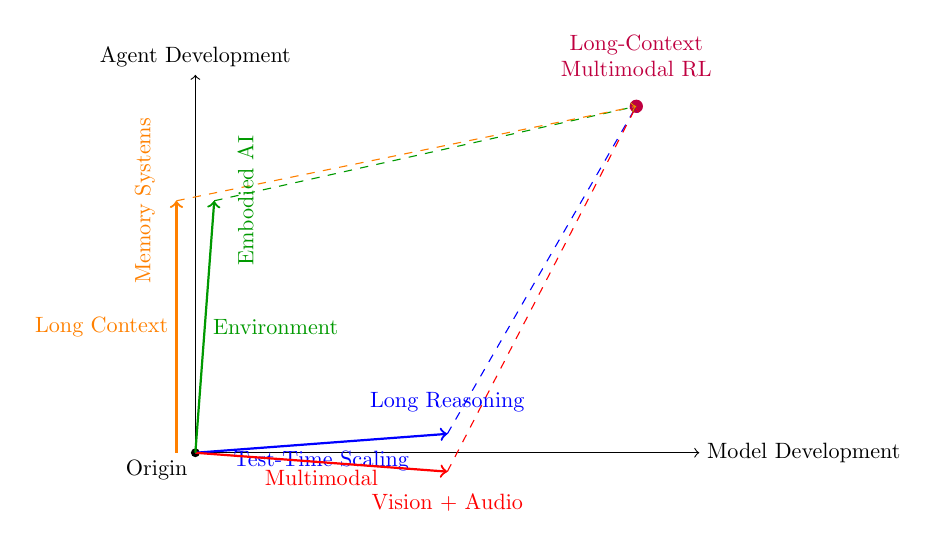
\begin{tikzpicture}[scale=0.8, every node/.style={scale=0.8}]
    % Axes
    \draw[->] (0,0) -- (8,0) node[right] {Model Development};
    \draw[->] (0,0) -- (0,6) node[above] {Agent Development};
    
    % Origin point
    \fill (0,0) circle (2pt) node[below left] {Origin};
    
    % Model development path (horizontal axis)
    \draw[->, thick, blue] (0,0) -- (4,0.3) node[midway, below] {Test-Time Scaling};
    \draw[->, thick, red] (0,0) -- (4,-0.3) node[midway, below] {Multimodal};
    
    % Agent development path (vertical axis)
    \draw[->, thick, green!60!black] (0,0) -- (0.3,4) node[midway, right] {Environment};
    \draw[->, thick, orange] (-0.3,0) -- (-0.3,4) node[midway, left] {Long Context};
    
    % Convergence point
    \fill[purple] (7,5.5) circle (3pt);
    \node[purple, align=center] at (7,6.3) {Long-Context\\Multimodal RL};
    
    % Connecting paths to convergence
    \draw[->, dashed, blue] (4,0.3) -- (7,5.5);
    \draw[->, dashed, red] (4,-0.3) -- (7,5.5);
    \draw[->, dashed, green!60!black] (0.3,4) -- (7,5.5);
    \draw[->, dashed, orange] (-0.3,4) -- (7,5.5);
    
    % Labels
    \node[blue] at (4,0.8) {Long Reasoning};
    \node[red] at (4,-0.8) {Vision + Audio};
    \node[green!60!black, rotate=90] at (0.8,4) {Embodied AI};
    \node[orange, rotate=90] at (-0.8,4) {Memory Systems};
\end{tikzpicture}
\end{center}
\end{frame}
